\documentclass[11pt,a4paper]{report}

\usepackage[utf8]{inputenc}
\usepackage[T1]{fontenc}

\pagestyle{empty}

\usepackage{graphicx} % Include figure files
\usepackage{amstext,amsbsy,amssymb}
%\usepackage{times} 

%% Numbered problems
\newcounter{excount}[chapter]
\newenvironment{exercise}[1][]{\addtocounter{excount}{1} \noindent {\bf Problem
    \arabic{excount} \ \ #1}\hspace{2mm}}{\vspace{4mm}}


\title{FYS3120 Classical Mechanics and Electrodynamics\\ 
\vspace{15mm}Problem set 2}


%%%%%%%
\begin{document}
%%%%%%%
\maketitle

%%%%%%%%
\begin{exercise}
Consider a general Lagrangian of the form $L=L(q_i,\dot q_i,t)$.

\begin{itemize}
\item[\bf a)] Explain the difference between the two types of time derivatives $\frac{dL}{dt}$ and $\frac{\partial L}{\partial t}$.
\item[\bf b)] Assume $q(t)=\{q_1(t),q_2(t),\ldots,q_d(t)\}$ is a solution of Lagrange's equations
\begin{equation}
\frac{d}{dt}\left(\frac{\partial L}{\partial \dot q_i}\right)-\frac{\partial L}{\partial q_i}=0,\quad i=1,2,\ldots,d.
\end{equation}
Show that for this solution, the following equation will be satisfied
\begin{equation}
\frac{d}{dt}\left(L-\sum_i\frac{\partial L}{\partial \dot q_i}\dot q_i\right)=\frac{\partial}{\partial t}L.
\end{equation}
\end{itemize}
\end{exercise}
%%%%%%%


%%%%%%%%
\begin{exercise}
Two identical rods of mass $m$ and length $l$ are connected to each other with a frictionless joint, see Fig.~\ref{fig:tworod}. The first rod is connected to a joint in the ceiling and to a joint at the center of the second rod. Assume that the motion takes place in the vertical plane. 
As a reminder the moment of inertia of a rod (with even mass distribution) about an endpoint is $I_1=ml^2/3$ and about the midpoint is $I_2=ml^2/12$.

%%%%%%%%%%
\begin{figure}[h!]
\begin{center}
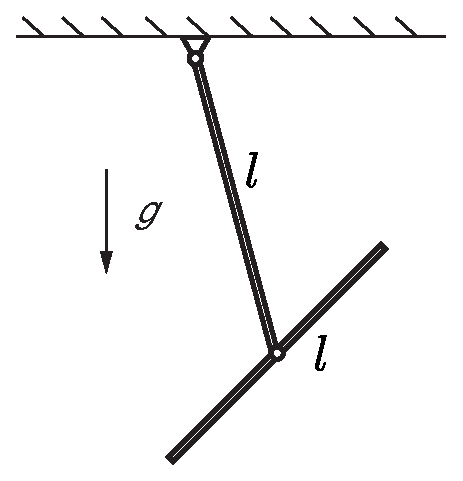
\includegraphics[width=4cm]{TwoRod.eps}
\end{center}
\caption{The two-rod problem.}
\label{fig:tworod}
\end{figure}
%%%%%%%%%% 

\begin{itemize}
\item[\bf a)] Choose suitable generalized coordinates for the system, and find the corresponding Lagrangian. 
\item[\bf b)] Formulate Lagrange's equations for the system, and find the angular frequency for small oscillations of the upper rod about its equilibrium position.
\end{itemize}
\end{exercise}
%%%%%%%


%%%%%%%%
\begin{exercise}
A small body with mass $m$ moves without friction on a rod, see Fig.~\ref{fig:rotatingrod}. The rod rotates in the horisontal plane, with constant angular velocity $\omega$ about a fixed point, which we assign the radial coordinate $r=0$. 

%%%%%%%%%%
\begin{figure}[h]
\begin{center}
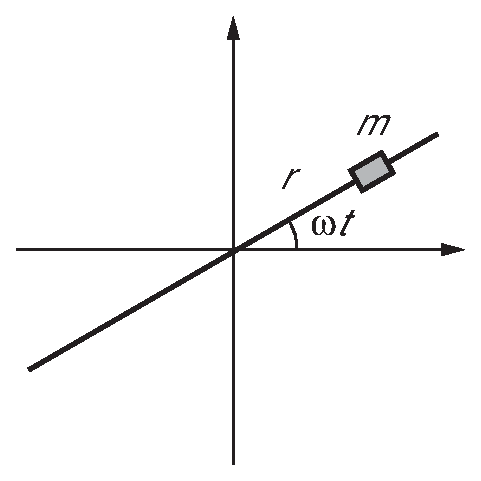
\includegraphics[width=4.4cm]{RotatingRod.eps}
\end{center}
\caption{Sliding body on a rotating rod.}
\label{fig:rotatingrod}
\end{figure}
%%%%%%%%%% 

\begin{itemize}
\item[\bf a)] Find Lagrange's equation for the radial coordinate $r$, and show that, with the initial condition $\dot r=0$ and $r=r_0$ at $t=0$, the equation has the solution $r=r_0\cosh{\omega t}$.
\item[\bf b)] Make a plot of the orbit in the horizontal $(x,y)$-plane, with dimensionless parameters $r_0=1$, $\omega=1$, and with $t$ restricted by $\omega t\lesssim \pi$. 
\end{itemize}
\end{exercise}
%%%%%%%


%%%%%%%%
\begin{exercise}
A pendulum consists of a rigid rod, which we consider as massless, and a pendulum bob of mass $m$. The point of suspension of the pendulum has horizontal coordinate $x=s$ and vertical coordinate $y=0$. This set-up is shown in Fig.~\ref{fig:pendulum}.

%%%%%%%%%%
\begin{figure}[h]
\begin{center}
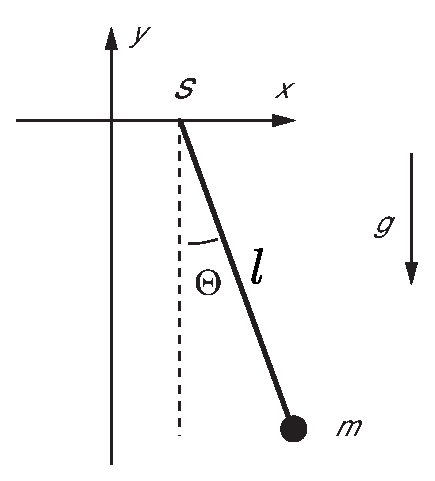
\includegraphics[width=4cm]{Pendulum.eps}
\end{center}
\caption{The pendulum problem.}
\label{fig:pendulum}
\end{figure}
%%%%%%%%%% 

\begin{itemize}
\item[\bf a)] Assume first that the point of suspension is kept fixed, with $s=0$. Use the angle $\theta$ as generalized coordinate, find the Lagrangian of the system and determine the form of Lagrange's equation for the system. Check that it has the standard form of a pendulum equation. 
\item[\bf b)] The point of suspension is now released so it can move freely in the horizontal direction ($x$-direction). Use $s$ and $\theta$ as generalized coordinates for the system and determine the corresponding set of Lagrange's equations. 
\item[\bf c)] Show that $s$ can be eliminated to give an equation which only depends on $\theta$ and its derivatives. Further show that this equation implies that the vertical motion of the pendulum bob is  identical to free fall in the gravitational field (in reality restricted by the length $l$ of the rod). 
\end{itemize}
\end{exercise}
%%%%%%%


\end{document}
%%%%%%%%%%
